\documentclass{article}
\usepackage[final]{neurips_2019}

% to avoid loading the natbib package, add option nonatbib:
%     \usepackage[nonatbib]{neurips_2019}

\usepackage[utf8]{inputenc} % allow utf-8 input
\usepackage[T1]{fontenc}    % use 8-bit T1 fonts
\usepackage{hyperref}       % hyperlinks
\usepackage{url}            % simple URL typesetting
\usepackage{booktabs}       % professional-quality tables
\usepackage{amsfonts}       % blackboard math symbols
\usepackage{nicefrac}       % compact symbols for 1/2, etc.
\usepackage{microtype}      % microtypography

\usepackage{amsmath}
\usepackage{graphicx}
\usepackage{float}
\usepackage{algorithm2e}
\usepackage{mdframed}
\usepackage[most]{tcolorbox}
\usepackage{subfig}
\usepackage{booktabs}
\renewcommand{\arraystretch}{1.2}  %make spacing of booktabs tables big

% Theorems
\usepackage{amsthm}
\renewcommand\qedsymbol{$\blacksquare$}
\makeatletter
\@ifclassloaded{article}{
    \newtheorem{definition}{Definition}[section]
    \newtheorem{example}{Example}[section]
    \newtheorem{theorem}{Theorem}[section]
    \newtheorem{corollary}{Corollary}[theorem]
    \newtheorem{lemma}{Lemma}[theorem]
}{
}
\makeatother

% Random Stuff
\setlength\unitlength{1mm}

\newcommand{\insertfig}[3]{
\begin{figure}[htbp]
\begin{center}
{\includegraphics[width=0.8 \textwidth]{#1}}
\end{center}
\caption{#2}\label{#3}
\end{figure}}

\newcommand{\insertxfig}[4]{
\begin{figure}[htbp]
\begin{center}
\leavevmode \centerline{\resizebox{#4\textwidth}{!}{\input
#1.pstex_t}}
\caption{#2} \label{#3}
\end{center}
\end{figure}}

\long\def\comment#1{}

\newcommand\norm[1]{\left\lVert#1\right\rVert}
\newcommand\abs[1]{\left\lvert#1\right\rvert}
\DeclareMathOperator*{\argmin}{arg\,min}
\DeclareMathOperator*{\argmax}{arg\,max}

% bb font symbols
\newfont{\bbb}{msbm10 scaled 700}
\newcommand{\CCC}{\mbox{\bbb C}}

\newfont{\bbf}{msbm10 scaled 1100}
\newcommand{\CC}{\mbox{\bbf C}}
\newcommand{\PP}{\mbox{\bbf P}}
\newcommand{\RR}{\mbox{\bbf R}}
\newcommand{\QQ}{\mbox{\bbf Q}}
\newcommand{\ZZ}{\mbox{\bbf Z}}
\renewcommand{\SS}{\mbox{\bbf S}}
\newcommand{\FF}{\mbox{\bbf F}}
\newcommand{\GG}{\mbox{\bbf G}}
\newcommand{\EE}{\mbox{\bbf E}}
\newcommand{\NN}{\mbox{\bbf N}}
\newcommand{\KK}{\mbox{\bbf K}}
\newcommand{\KL}{\mbox{\bbf KL}}
\newcommand{\MM}{\mbox{\bbf M}}

% Vectors
\renewcommand{\aa}{{\bf a}}
\newcommand{\bb}{{\bf b}}
\newcommand{\cc}{{\bf c}}
\newcommand{\dd}{{\bf d}}
\newcommand{\ee}{{\bf e}}
\newcommand{\ff}{{\bf f}}
\renewcommand{\gg}{{\bf g}}
\newcommand{\hh}{{\bf h}}
\newcommand{\ii}{{\bf i}}
\newcommand{\jj}{{\bf j}}
\newcommand{\kk}{{\bf k}}
\renewcommand{\ll}{{\bf l}}
\newcommand{\mm}{{\bf m}}
\newcommand{\nn}{{\bf n}}
\newcommand{\oo}{{\bf o}}
\newcommand{\pp}{{\bf p}}
\newcommand{\qq}{{\bf q}}
\newcommand{\rr}{{\bf r}}
\renewcommand{\ss}{{\bf s}}
\renewcommand{\tt}{{\bf t}}
\newcommand{\uu}{{\bf u}}
\newcommand{\ww}{{\bf w}}
\newcommand{\vv}{{\bf v}}
\newcommand{\xx}{{\bf x}}
\newcommand{\yy}{{\bf y}}
\newcommand{\zz}{{\bf z}}
\newcommand{\0}{{\bf 0}}
\newcommand{\1}{{\bf 1}}

% Matrices
\newcommand{\Ab}{{\bf A}}
\newcommand{\Bb}{{\bf B}}
\newcommand{\Cb}{{\bf C}}
\newcommand{\Db}{{\bf D}}
\newcommand{\Eb}{{\bf E}}
\newcommand{\Fb}{{\bf F}}
\newcommand{\Gb}{{\bf G}}
\newcommand{\Hb}{{\bf H}}
\newcommand{\Ib}{{\bf I}}
\newcommand{\Jb}{{\bf J}}
\newcommand{\Kb}{{\bf K}}
\newcommand{\Lb}{{\bf L}}
\newcommand{\Mb}{{\bf M}}
\newcommand{\Nb}{{\bf N}}
\newcommand{\Ob}{{\bf O}}
\newcommand{\Pb}{{\bf P}}
\newcommand{\Qb}{{\bf Q}}
\newcommand{\Rb}{{\bf R}}
\newcommand{\Sb}{{\bf S}}
\newcommand{\Tb}{{\bf T}}
\newcommand{\Ub}{{\bf U}}
\newcommand{\Wb}{{\bf W}}
\newcommand{\Vb}{{\bf V}}
\newcommand{\Xb}{{\bf X}}
\newcommand{\Yb}{{\bf Y}}
\newcommand{\Zb}{{\bf Z}}

% Calligraphic
\newcommand{\Ac}{{\cal A}}
\newcommand{\Bc}{{\cal B}}
\newcommand{\Cc}{{\cal C}}
\newcommand{\Dc}{{\cal D}}
\newcommand{\Ec}{{\cal E}}
\newcommand{\Fc}{{\cal F}}
\newcommand{\Gc}{{\cal G}}
\newcommand{\Hc}{{\cal H}}
\newcommand{\Ic}{{\cal I}}
\newcommand{\Jc}{{\cal J}}
\newcommand{\Kc}{{\cal K}}
\newcommand{\Lc}{{\cal L}}
\newcommand{\Mc}{{\cal M}}
\newcommand{\Nc}{{\cal N}}
\newcommand{\Oc}{{\cal O}}
\newcommand{\Pc}{{\cal P}}
\newcommand{\Qc}{{\cal Q}}
\newcommand{\Rc}{{\cal R}}
\newcommand{\Sc}{{\cal S}}
\newcommand{\Tc}{{\cal T}}
\newcommand{\Uc}{{\cal U}}
\newcommand{\Wc}{{\cal W}}
\newcommand{\Vc}{{\cal V}}
\newcommand{\Xc}{{\cal X}}
\newcommand{\Yc}{{\cal Y}}
\newcommand{\Zc}{{\cal Z}}

% Bold greek letters
\newcommand{\alphab}{\hbox{\boldmath$\alpha$}}
\newcommand{\betab}{\hbox{\boldmath$\beta$}}
\newcommand{\gammab}{\hbox{\boldmath$\gamma$}}
\newcommand{\deltab}{\hbox{\boldmath$\delta$}}
\newcommand{\etab}{\hbox{\boldmath$\eta$}}
\newcommand{\lambdab}{\hbox{\boldmath$\lambda$}}
\newcommand{\epsilonb}{\hbox{\boldmath$\epsilon$}}
\newcommand{\nub}{\hbox{\boldmath$\nu$}}
\newcommand{\mub}{\hbox{\boldmath$\mu$}}
\newcommand{\zetab}{\hbox{\boldmath$\zeta$}}
\newcommand{\phib}{\hbox{\boldmath$\phi$}}
\newcommand{\psib}{\hbox{\boldmath$\psi$}}
\newcommand{\thetab}{\hbox{\boldmath$\theta$}}
\newcommand{\taub}{\hbox{\boldmath$\tau$}}
\newcommand{\omegab}{\hbox{\boldmath$\omega$}}
\newcommand{\xib}{\hbox{\boldmath$\xi$}}
\newcommand{\sigmab}{\hbox{\boldmath$\sigma$}}
\newcommand{\pib}{\hbox{\boldmath$\pi$}}
\newcommand{\rhob}{\hbox{\boldmath$\rho$}}

\newcommand{\Gammab}{\hbox{\boldmath$\Gamma$}}
\newcommand{\Lambdab}{\hbox{\boldmath$\Lambda$}}
\newcommand{\Deltab}{\hbox{\boldmath$\Delta$}}
\newcommand{\Sigmab}{\hbox{\boldmath$\Sigma$}}
\newcommand{\Phib}{\hbox{\boldmath$\Phi$}}
\newcommand{\Pib}{\hbox{\boldmath$\Pi$}}
\newcommand{\Psib}{\hbox{\boldmath$\Psi$}}
\newcommand{\Thetab}{\hbox{\boldmath$\Theta$}}
\newcommand{\Omegab}{\hbox{\boldmath$\Omega$}}
\newcommand{\Xib}{\hbox{\boldmath$\Xi$}}

% mixed symbols
\newcommand{\sinc}{{\hbox{sinc}}}
\newcommand{\diag}{{\hbox{diag}}}
\renewcommand{\det}{{\hbox{det}}}
\newcommand{\trace}{{\hbox{tr}}}
\newcommand{\tr}{\trace}
\newcommand{\sign}{{\hbox{sign}}}
\renewcommand{\arg}{{\hbox{arg}}}
\newcommand{\var}{{\hbox{var}}}
\newcommand{\cov}{{\hbox{cov}}}
\renewcommand{\Re}{{\rm Re}}
\renewcommand{\Im}{{\rm Im}}
\newcommand{\eqdef}{\stackrel{\Delta}{=}}
\newcommand{\defines}{{\,\,\stackrel{\scriptscriptstyle \bigtriangleup}{=}\,\,}}
\newcommand{\<}{\left\langle}
\renewcommand{\>}{\right\rangle}
\newcommand{\Psf}{{\sf P}}
\newcommand{\T}{\top}
\newcommand{\m}[1]{\begin{bmatrix} #1 \end{bmatrix}}


\usepackage[final]{pdfpages}

\title{Differential Geometry Midterm Project}
\author{%
 Tim Player \\
  Harvey Mudd College\\
  Claremont, CA 91711 \\
  \texttt{tplayer@hmc.edu} \\
}

\begin{document}
\maketitle

\begin{abstract}
    This is where I will put my abstract.
\end{abstract}

\section{Motivation}
Precisely localizing moving platforms using inertial sensors is a fundamental problem in robotics. These sensors, such as gyroscopes, accelerometers, and magnetometers, allow changes in position and orientation (together, ``pose") to be determined over short time scales in a process called \textit{dead reckoning}. This approach is used, for instance, in aerospace where precise estimates of aircraft pose may lead to safer landings. However, the cheapest sensors provide noisy measurements which cause dead-reckoning to be generally ineffective over long periods of time. 

MEMS magnetometers, which are used as digital compasses to provide estimates of orientation with respect to the Earth's magnetic field, can provide erroneous estimates due to the presence of magnetic material near the sensor, unmodeled geological perturbations in the Earth's field, miscalibration, and white observation noise. This can lead to uncertainty in orientation measurements on the order of several degrees (\cite{introtoor}). The error, in turn, causes exponentially-growing errors in position estimation, as we will discuss in Section \ref{sec:poseest}. As a result, absolute measurements of orientation which are independent of magnetometers have direct utility in robotic state estimation.

This project implements direct orientation measurement via computer vision horizon estimation. Using inertial and visual data collected on a supersonic sounding rocket in April 2019, we develop an algorithm for pose estimation which incorporates visual horizon estimation as an independent, redundant measure of orientation to address the deficiencies of magnetometers. As shown in Fig. \ref{fig:horizon_overview}, cameras mounted inside of the rocket face opposite directions so they can see the horizon. As a result, changes in rocket attitude manifest in the camera image as coupled and opposite tilting, raising, or lowering of the horizon in each image. This allows direct estimation of pitch and yaw in a global frame.

In this paper, we first provide an explicit overview of the pose-estimation problem in section \ref{sec:posest} and detail some existing algorithms. In section \ref{sec:dynmod}, we develop the dynamical model used to represent the physical constraints of the rocket trajectory. Section \ref{sec:data} presents in more depth the available data collected during the April flights and the steps needed to prepare it for use in a sensor fusion algorithm. Lastly, section \ref{sec:algorithm} gives an overview of the multiplicative Extended Kalman Filter we use, including the parametrization of orientation with unit quaternions.

%%%%%%%%%%%%%%%%%%%%%%%%%%%%   FIGURE  %%%%%%%%%%%%%%%%%%
\begin{figure}[ht]%
 \centering
 \subfloat[]{\includegraphics[width=5cm]{rocket_fov2.jpg}\label{fig:a}}\\
 \subfloat[]{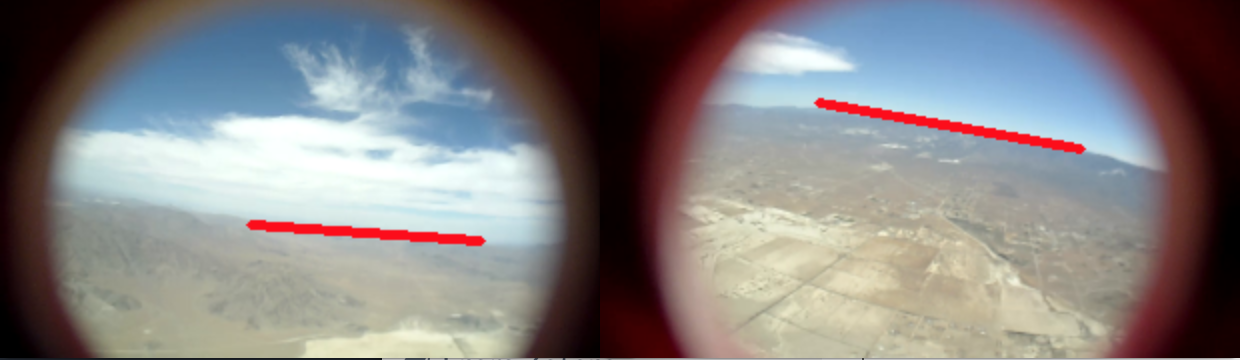
\includegraphics[width=5cm]{horiz.png}\label{fig:b}}%
 \caption{Visual horizon identification scheme during rocket flight. Approximate field of view of opposite-facing cameras is shown in red in sub-figure (a). Camera output is shown in sub-figure (b).}%
 \label{fig:horizon_overview}%
\end{figure}
%%%%%%%%%%%%%%%%%%%%%%%%%%%%%%%%%%%%%%%%%%%%%%%%%%%%%%%%%

\section{Pose Estimation Problem} \label{sec:posest}
The problem of \textit{sensor fusion} comprises strategies to intelligently combine observations from the various sensors which indirectly measure different elements of the platform's pose. Whereas the system's pose includes
\[
\{\text{\textit{x}-position,\textit{y}-position, \textit{z}-position, pitch, roll, yaw}\}
= \{x, y, z, r, p, y\},
\]
direct measurements of these items are not available. The gyroscope, for instance, observes the time-derivatives $\{\dot{r}, \dot{p}, \dot{y}\}$, and the accelerometer measures \textit{specific force}, which provides gravity-biased measurements of $\{\ddot{x}, \ddot{y}, \ddot{z} \}$ in a local frame. As discussed above, magnetometers provide a noisy absolute measurement of the orientation $\{r, p, y\}$. 

It is necessary to define several frames of reference. First, the \textit{body} frame $\textbf{b}$ is the coordinate frame of the moving rocket. This has the pitch axis $x_b$, yaw axis $y_b$, and roll axis $z_b$ shown in Fig. \ref{fig:axes}. 

The navigation frame $\textbf{n}$ is the coordinate frame in which we wish to localize the rocket, whose origin is at the launch pad. To this we ascribe the North, East, Down (NED) triad. Note that both systems described have positive orientation. 

To be fully comprehensive, we must also include the \textit{inertial} frame \textbf{i} and the \textit{Earth} frame \textbf{e}. The accelerometer and rate gyroscope take measurements with respect to the inertial frame rather than the navigation frame or body frame, and thus the effects of Coriolis acceleration caused by the Earth's rotation and body acceleration caused by the Earth's orbit may be factored in. However, as the rocket flight is on the order of minutes, the frames do not become significantly different so we make the valid simplifying assumption that the navigation frame \textbf{n} is inertial, and we remove \textbf{i} and \textbf{e} from further discussion.

%%%%%%%%%%%%%%%%%%%%%%%%%%%%   FIGURE  %%%%%%%%%%%%%%%%%%
\begin{figure}[htbp]%
    \centering
      	\framebox{
            \subfloat{
                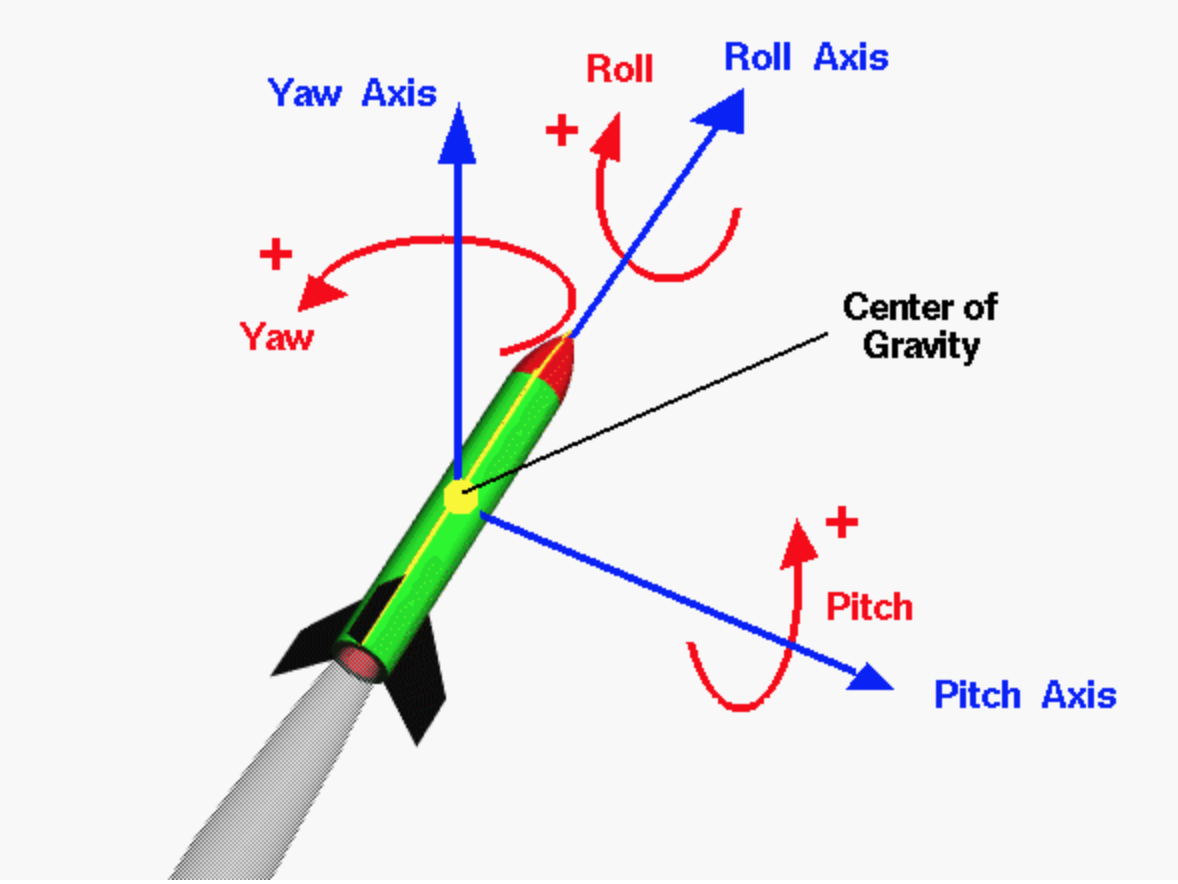
\includegraphics[width=8cm]{rotations.png} 
            }
        }
    \caption{Attitude axis conventions. Camera 1's aperture lies on the pitch axis.}%
    \label{fig:axes}
\end{figure}
%%%%%%%%%%%%%%%%%%%%%%%%%%%%%%%%%%%%%%%%%%%%%%%%%%%%%%%%%

To achieve a pose in the navigation frame based on measurements taken in the body frame, we must correct for the presence of gravity in the accelerometer measurements prior to integrating. As shown in Fig. \ref{fig:dr}, the rocket's orientation is first estimated via direct measurement with the magnetometer and by integrating of rate gyroscope values from the last time step. With this known orientation — a rotation between the \textbf{b} and \textbf{n} frames — the direction of gravity is known. Then gravity can be subtracted from the accelerometer readings to provide a measurement of true rocket acceleration in the navigation frame rather than specific force. Lastly, this acceleration is integrated twice to arrive at velocity and position.

\begin{figure}[ht]
  \centering
  \fbox{
  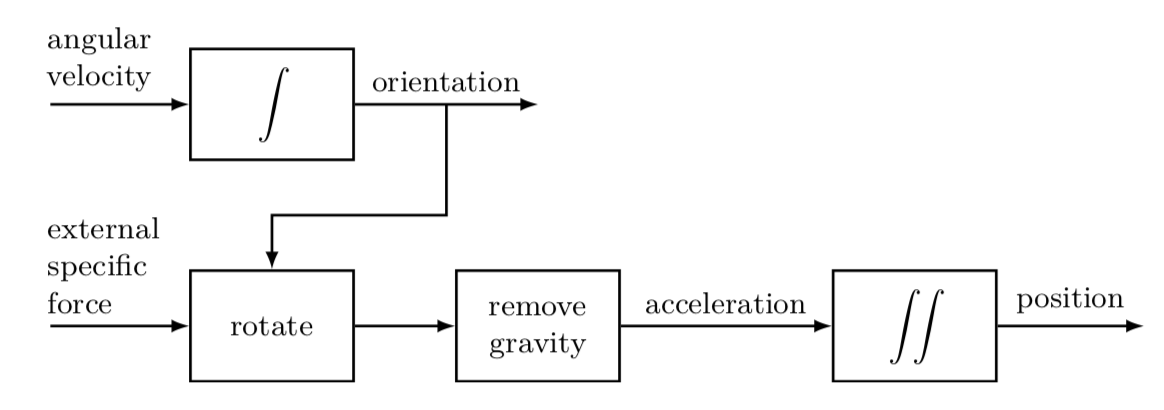
\includegraphics[width=0.7\textwidth]{dr.png}
    }
  \caption{Schematic illustration of dead-reckoning, where the accelerometer measurements (external specific force) and the gyroscope measurements (angular velocity) are integrated to position and orientation. From \cite{1}.}
  \label{fig:dr}
\end{figure}

To estimate pose, our approach to dead reckoning must intelligently utilize all data. Specifically, at each step $t$ along the rocket's trajectory we seek to quantify a conditional belief distribution regarding the rocket's pose $x_t$
\[ \label{eq:cond}
bel(t) = p(x_t | z_{1:t}),
\]
where $z_{1:t}$ are all of the measurements available from sensors through times $1$ through $t$. Under the Markov assumption, which is that our description of the rocket's state is complete enough that the knowledge of a prior state specifies belief of future states as well, then Eq. \ref{eq:cond} reduces to
\[
bel(t) = p(x_t | x_{t-1}, z_t),
\]
which is to say that the information from all measurements $z_{1:t-1}$ is included in the state $x_{t-1}$. This forms the basis of the Bayes Filter in general. We will implement a specific closed-form solution of the Bayes Filter in section \ref{sec:algorithm}.

\section{Dynamical Model} \label{sec:dynmod}
We use a kinematic model without considering a forcing input $u$. While a linear dynamical system in general is defined by 
\begin{align*}
\frac{d}{dt} x = A x + B u\\
y = C x + D u
\end{align*}
Where $A \in \MM_{n \times n}$ is the system dynamics matrix, $B \in \MM_{n \times m}$ is the input matrix, $C \in \MM_{r \times n}$ is the output matrix, and $D \in \MM_{r \times m}$ is the transmission matrix. These matrices relate the state $x$ and input $y$ to its derivative.

In the discrete time case, as implemented in digital systems, we replace $A$ with $A_d = e^{AT}$, where $T$ is the time step. As mentioned above, we entirely neglect $u$. However, we assume the presence of Gaussian noise in our state measurements.

As in \cite{introtoiner}, we choose to parametrize orientation via quaternions, as we discuss in section \ref{sec:algorithm}. We borrow the dynamics equations from [\cite{introtoiner}] to relate the position $p_t^n$, velocity $v_t^n$, and orientation are related to the measured acceleration and gyroscope inputs via
\begin{figure}[ht]
  \centering
  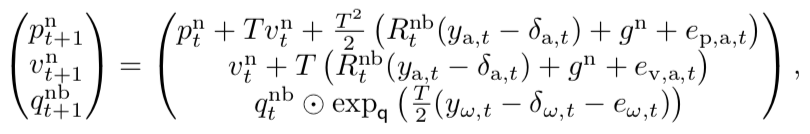
\includegraphics[width=0.7\textwidth]{dynamics.png}
\end{figure}

where
\begin{figure}[ht]
  \centering
  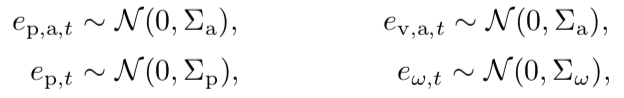
\includegraphics[width=0.6\textwidth]{dynamics2.png}
\end{figure}

with $\Sigma_a = \sigma_a^2 I_3$ and $\Sigma_2 = \sigma_w^2 I_3$. Then, the problem becomes to estimate the state using known time series data $y_{a_t}$ and $y_{\omega,t}$ for each step $t$.

Additionally, measurements of orientation are available from the magnetometer as
\begin{figure}[ht]
  \centering
  
\includegraphics[width=0.3\textwidth]{dynamics3.png}
\end{figure}

We must also incorporate the yaw measurements from the cameras.

\section{Data Handling} \label{sec:data}
Our data-processing pipeline must include the following.
\begin{enumerate}
    \item Find initial GPS location on the launch pad.
    \item Convert GPS data (not available during ascent) into meters from origin
    \item Apply laboratory bias-calibrations to raw accelerometer, gyroscope, and magnetometer data.
    \item Flip magnetometer $x$, $y$ aces to get right-handed system
    \item Scale magnetometer dimensions individually to normalize to $(-1, 1)$.
    \item Scale magnetometer readings so that at every step $t$ the $L_2$ norm is $1$.
    \item Get initial magnetometer orientation from the pre-launch sample mean. Also get sensor variance.
    \item Resample magnetometer using smooth interpolation.
    \item Convert gyroscope data to radians/sec.
    \item Convert accelerometer data to meters/sec using local gravitational constant.
    \item Get acceleration baseline from pre-launch sample mean. Also get sensor variance.
    \item Resample accelerometer and gyroscope data.
    \item \label{camerastep}Determine the global pitch and yaw corresponding to each image.
    \item Smooth the roll using complementary filter.
    \item Determine initial orientation using TRIAD method.
\end{enumerate}
This sequence of pre-processing steps should yield a unified set of relevant time-series data for sensor fusion. However, item \ref{camerastep} deserves more elaboration. We do so below. 

\subsection{Estimating Pitch and Yaw from Images}

The problem of estimating the rocket's attitude from camera output is governed by the underlying projective geometry of the camera-world system. Consider the elementary graphics equation relating individual points in 3D space to camera pixels,
\begin{align}
\label{eq:cam}
\mathbf{y} &= f(\mathbf{x}) \\
&= H (R | \mathbf{t}) \mathbf{x}.
\end{align}
Here, $\mathbf{y} = (x_{image}, y_{image}, 1)^T$ gives the position of the image on the camera plane, and is a function of $\mathbf{x} = (x_{object}, y_{object}, z_{object}, 1)^T$, the position of the object. $H$ is the lens distortion matrix relating points on the ideal image plane to the actual pixel output. $R$ is the rotation matrix between the camera orientation and global coordinates, and $\mathbf{t}$ is the translation vector $(x, y, z, 1)^T$ defining the position of the camera.

Eq. \ref{eq:cam} , implies a general approach to the problem of visual pose estimation. The camera pose matrix $(R | \mathbf{t})$, which is an element of $M_{4\times3}$, may be estimated by the correct identification of five spatially distinct features. This technique is known as ``direct linear transformation". That approach, which is akin to triangulation, is subject to the same sensitivity problem as conventional 2D triangulation: the features must be separated by a large angular distance in order to properly identify the camera pose within reasonable error. The addition of more point pairs increases the certainty of the estimation.

The problem of extracting the pose of a camera from a single view is common in the computer vision and robotics literature, and the general approach described above has been efficiently implemented in the limiting case of structure-from-motion as ``visual odometry" and ``visual simultaneous localization and mapping". These approaches are very clever, but we implemented a simpler scheme to recover only pitch and yaw instead of the full pose.

By inspection of Figure \ref{fig:axes}, it can be seen that the slope and height of the horizon in a camera image represent respectively the pitch and yaw of the rocket. If the rocket pitches into the page, then the horizon will slope clockwise in the starboard camera image, and if the rocket yaws to the left, then the horizon will rise in the page; the opposite is true for the port camera. 

We make the simplification that the lens distortion matrix $H$ can be neglected, which is reasonable given that the fisheye lens results in only minimal distortion of lines passing near the center of the image (Fig. \ref{fig:horizon_overview}. Thus, in theory, raw camera output can be converted to rocket pitch and yaw measurements by identifying the slope and height of the horizon in the image, inferring the corresponding camera attitude, and correcting for the relative rotation between the camera and rocket.

\subsection{Computer Vision Algorithm for Horizon Estimation}
An algorithm to automatically detect the horizon was implemented in OpenCV. The algorithm works by translating the image to an HSV (hue, saturation, and value) colorspace and identifying the sky. The edges of the sky region are then identified, and a straight line is fitted to the horizon. More specifically, the algorithm
\begin{enumerate}
    \item Makes a mask that includes the sky but not the ground, using an HSV tranform and thresholding.
    \item Finds the edges of that mask using Canny edge detection.
    \item Picks the longest edge. Assumes that contains the horizon.
    \item Crops the image to only examine the central rectangle (and not the edges of the circular window).
    \item Uses Hough line transform to identify a long straight line.
\end{enumerate}

An example set of computer vision intermediate steps is shown in Fig. \ref{fig:cv_alg}.

%%%%%%%%%%%%%%%%%%%%%%%%%%%%   FIGURE  %%%%%%%%%%%%%%%%%%
\begin{figure}[H]%
 \centering
 \subfloat[]{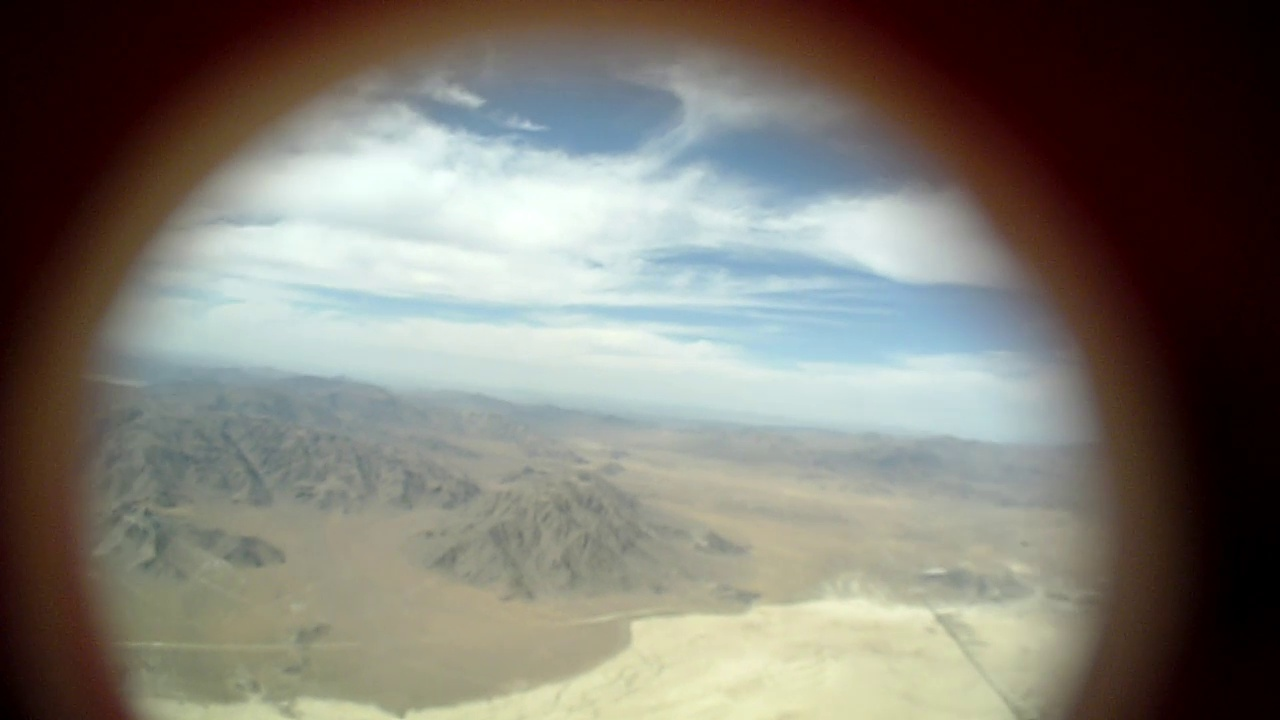
\includegraphics[width=3cm]{frame1_r.jpg}}\\
 \subfloat[]{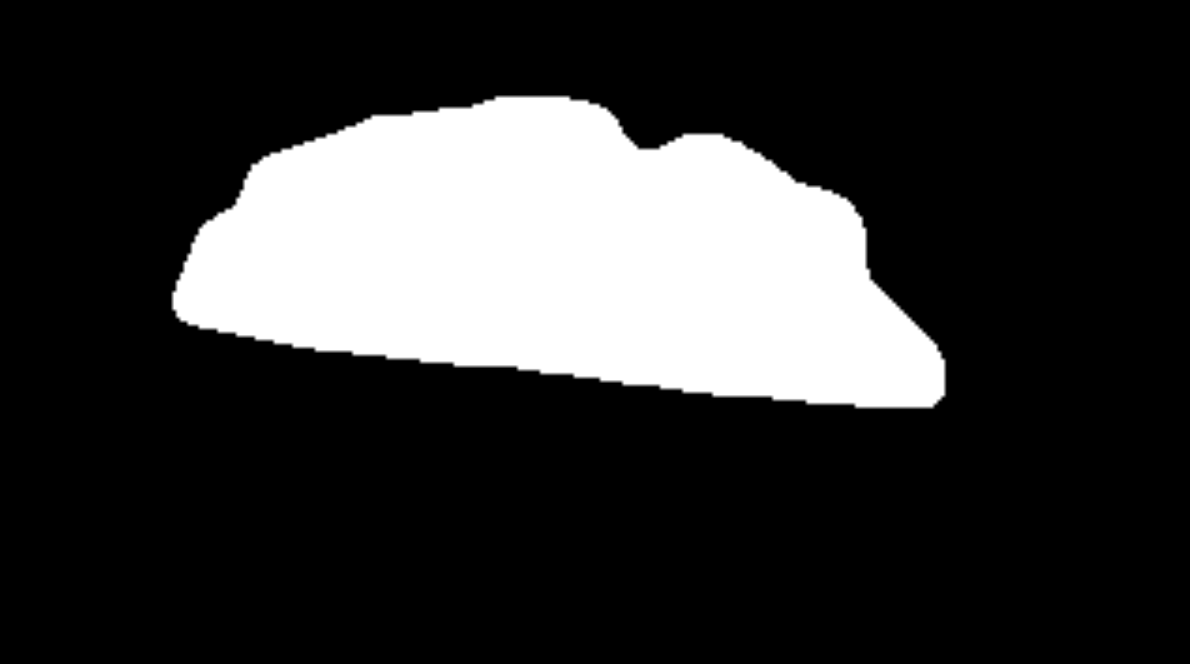
\includegraphics[width=3cm]{mask.png}}%
 \subfloat[]{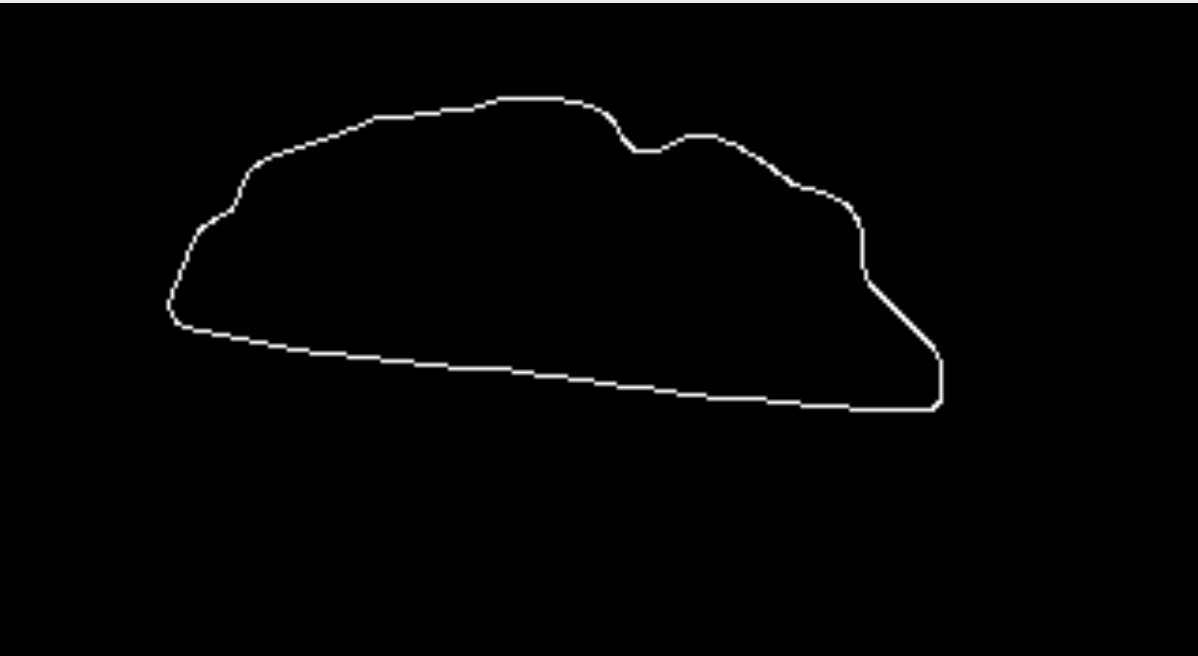
\includegraphics[width=3.1cm]{edges.png}}\\
 \subfloat[]{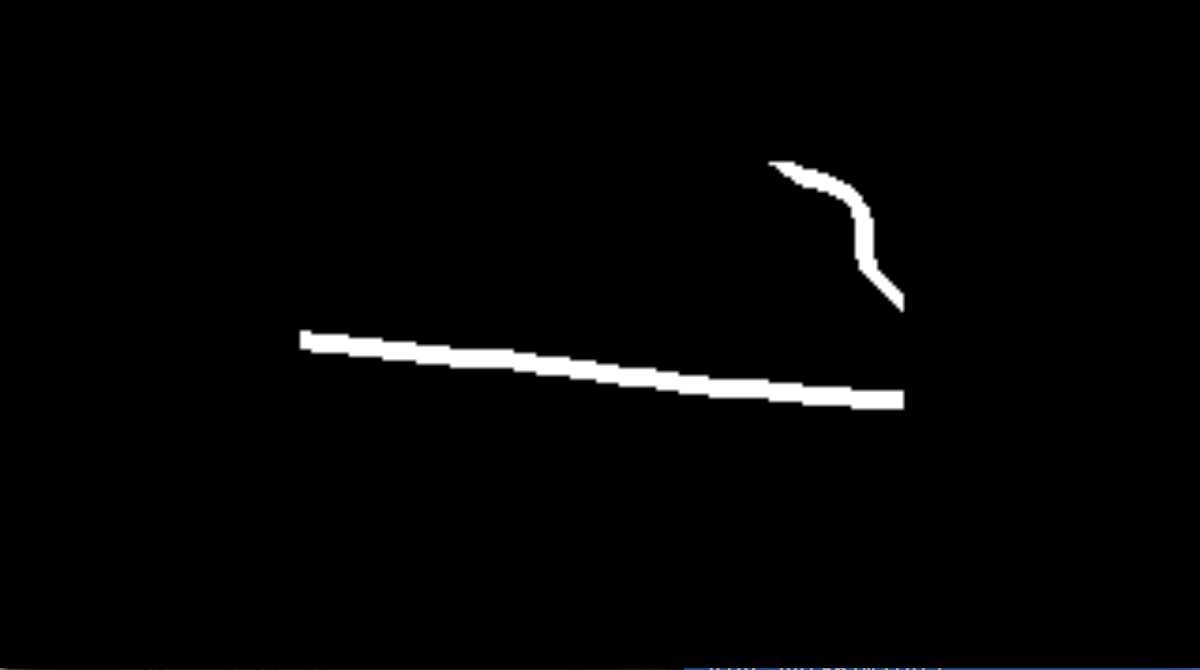
\includegraphics[width=3.1cm]{hcont.png}}%
 \subfloat[]{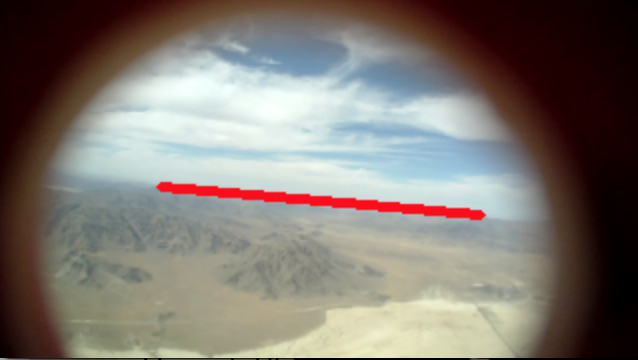
\includegraphics[width=3cm]{frame1.png}}%
 \caption{Computer vision algorithm for identifying the horizon in an image.}%
 \label{fig:cv_alg}%
\end{figure}
%%%%%%%%%%%%%%%%%%%%%%%%%%%%%%%%%%%%%%%%%%%%%%%%%%%%%%%%%

\section{Algorithm} \label{sec:algorithm}
We will use the multiplicative Extended Kalman Filter with a quaternion orientation estimation, as below [\cite{introtoiner}].

\begin{figure}[ht]
  \centering
  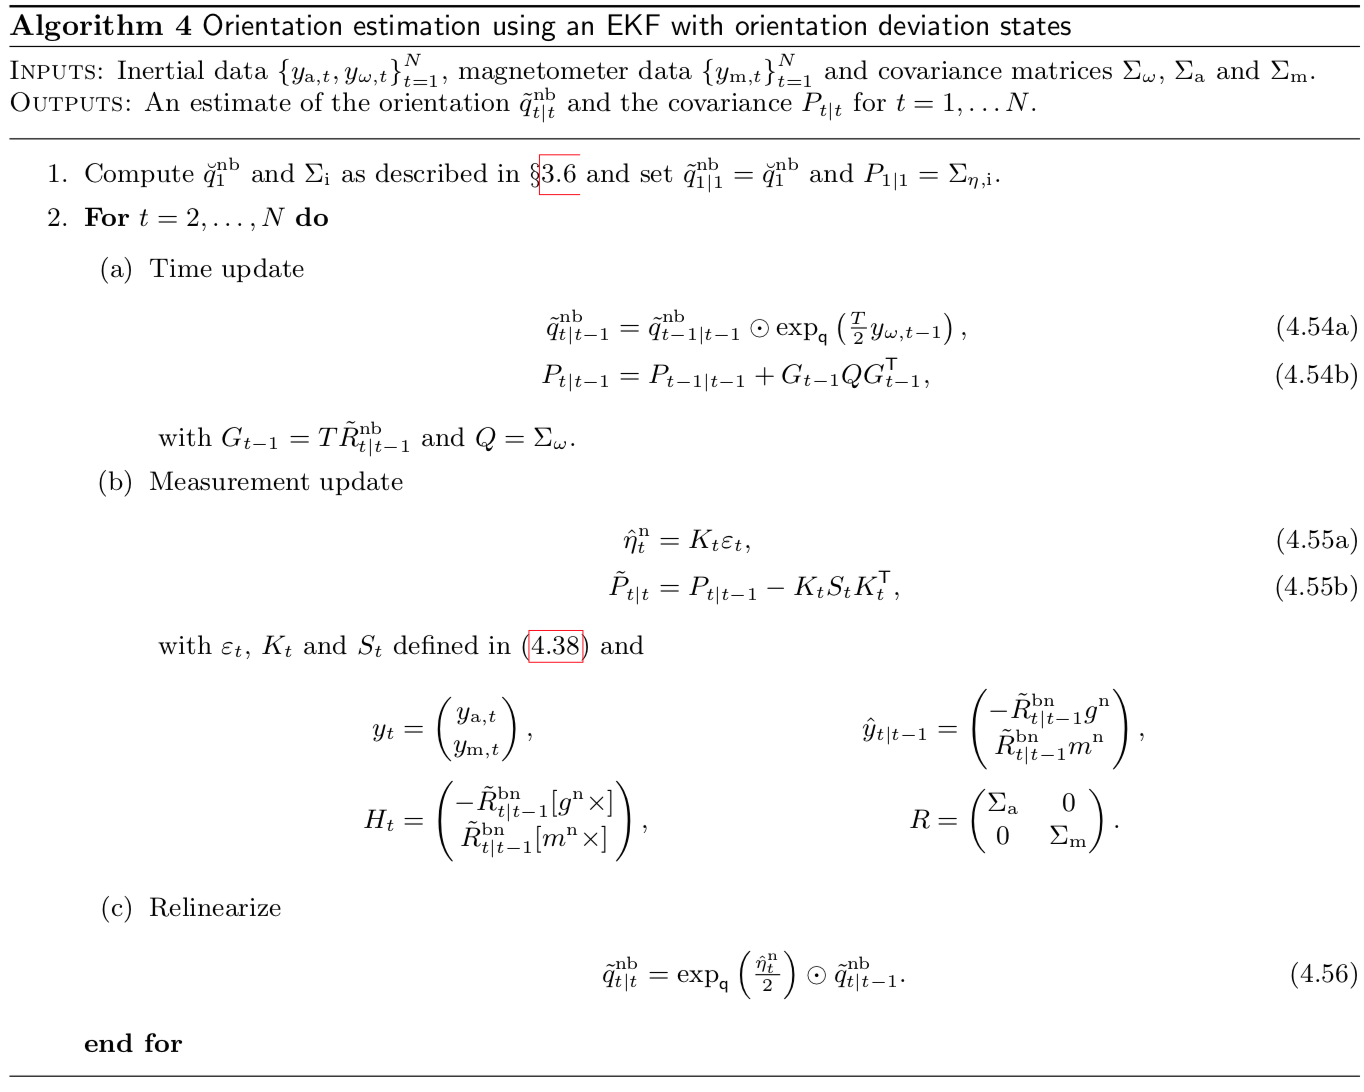
\includegraphics[width=0.9\textwidth]{algo.png}
\end{figure}


\begin{thebibliography}{}
Unfortunately, I did not have time to cite my sources for this interim midterm review. I look forward to citing these invaluable authors -- including primarily Erik Spjut, Manon Kok, Jeroen D. Hol, Thomas B. Schon, Sebastian Thrun, Wolfram Burgard, and Dieter Fox, in greater detail for my final project.

\end{thebibliography}
%\subsection{Quaternion Orientation Parametrization}
\end{document}
